\beginsong{Unter den Toren}[wuw={olka (Erich Scholz), mac (Erik Martin)}, pfii={29}, pfiii={14}, bo={338}, gruen={162}, kssiv={12}]

\beginverse
\endverse 
\centering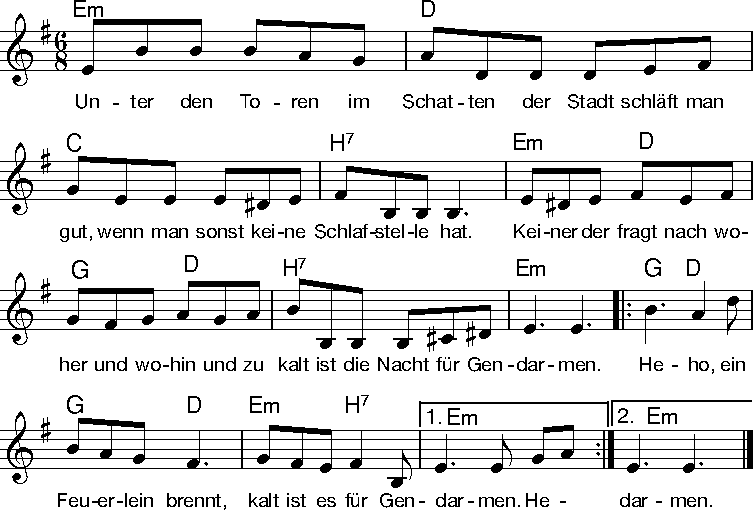
\includegraphics[width=1\textwidth]{Noten/Lied090.pdf}

\beginverse
\[Em]Silberne Löffel und \[D]Ketten im Sack legst du \[C]besser beim Schlafen dir 
\[H7]unters Genack. \[Em]Zeig' nichts und \[D]sag nichts, die \[G]Messer sind \[D]stumm 
und zu \[H7]kalt ist die Nacht für Gen\[Em]darmen.
\endverse

\beginchorus
\lrep \[G]He\[D]-jo, ein \[G]Feuerlein \[D]brennt, \[Em]kalt ist es \[H7]für Gen\[Em]darmen. \rrep
\endchorus

\beginverse
^Greif' nach der Flasche, doch ^trink' nicht zu viel deine ^Würfel sind gut,
aber ^falsch ist das Spiel. ^Spuck in die ^Asche und ^schau' lieber ^zu denn zu ^kalt ist die Nacht für Gen^darmen. 
\endverse
%\renewcommand{\everychorus}{\textnote{\bf Refrain (wdh.)}}

\beginchorus
\lrep \[G]He\[D]-jo, ein \[G]Feuerlein \[D]brennt, \[Em]kalt ist es \[H7]für Gen\[Em]darmen. \rrep
\endchorus


\beginverse
^Rückt dir die freundliche ^Schwester zu nah, das ist ^gut für die
Wärme mal ^hier und mal da. ^Keiner im ^Dunkeln ver^rät sein
Ge^sicht und zu ^kalt ist die Nacht für Gen^darmen.
\endverse

\beginchorus
\lrep \[G]He\[D]-jo, ein \[G]Feuerlein \[D]brennt, \[Em]kalt ist es \[H7]für Gen\[Em]darmen. \rrep
\endchorus

\beginverse
^Geh' mit der Nacht, eh der ^Frühnebel steigt, nur das ^Feuer bleibt stumm
und das ^Scheit, das verschweigt. ^Lass' nichts zu^rück und ver^giss', was
du ^sahst, denn die ^Sonne bringt bald die Gen^darmen.
\endverse
%\renewcommand{\everychorus}{\textnote{\bf Refrain}}

\beginchorus
\lrep \[G]He\[D]-jo, das \[G]Feuer ist \[D]aus, \[Em]bald kommen \[H7]die Gen\[Em]darmen. \rrep
\endchorus

\endsong

\beginscripture{} 
Gendarm = Wachmann
\endscripture

\begin{intersong}
%\centering\includegraphics[width=0.5\textwidth]{Bilder/MorphieVorFeuerSchatten.png}	
%\ThisLRCornerWallPaper{0.7}{Bilder/MorphieVorFeuerSchatten.png}
%\ThisLRCornerWallPaper{0.7}{Bilder/MorphieVorFeuer.png}
\end{intersong}